\documentclass[12pt]{article}

\newcommand{\CiteMathPackage}{../Notes/math}
\newcommand{\CiteReference}{../Notes/reference.bib}

% Packages
\usepackage{setspace,geometry,fancyvrb,rotating}
\usepackage{marginnote,datetime,enumitem}
\usepackage{titlesec,indentfirst}
\usepackage{amsmath,amsfonts,amssymb,amsthm,mathtools}
\usepackage{threeparttable,booktabs,adjustbox}
\usepackage{graphicx,epstopdf,float,soul,subfig}
\usepackage[toc,page]{appendix}
\usdate

% Page Setup
\geometry{scale=0.8}
\titleformat{\paragraph}[runin]{\itshape}{}{}{}[.]
\titlelabel{\thetitle.\;}
\setlength{\parindent}{10pt}
\setlength{\parskip}{10pt}
\usepackage{Alegreya}
\usepackage[T1]{fontenc}

%% Bibliography
\usepackage{natbib,fancybox,url,xcolor}
\definecolor{MyBlue}{rgb}{0,0.2,0.6}
\definecolor{MyRed}{rgb}{0.4,0,0.1}
\definecolor{MyGreen}{rgb}{0,0.4,0}
\definecolor{MyPink}{HTML}{E50379}
\newcommand{\highlightR}[1]{{\emph{\color{MyRed}{#1}}}} 
\newcommand{\highlightB}[1]{{\emph{\color{MyBlue}{#1}}}}
\newcommand{\highlightP}[1]{{\emph{\color{MyPink}{#1}}}}
\usepackage[bookmarks=true,bookmarksnumbered=true,colorlinks=true,linkcolor=MyBlue,citecolor=MyRed,filecolor=MyBlue,urlcolor=MyGreen]{hyperref}
\bibliographystyle{econ}

%% Theorem Environment
\theoremstyle{definition}
\newtheorem{assumption}{Assumption}
\newtheorem{definition}{Definition}
\newtheorem{theorem}{Theorem}
\newtheorem{proposition}{Proposition}
\newtheorem{lemma}[theorem]{Lemma}
\newtheorem{example}[theorem]{Example}
\newtheorem{corollary}[theorem]{Corollary}
\usepackage{mathtools}
\usepackage{\CiteMathPackage}


\begin{document}

%??%??%??%??%??%??%??%??%??%??%??%??%??%??%??%??%??%??%??%??%??%??
%?? title 
%??%??%??%??%??%??%??%??%??%??%??%??%??%??%??%??%??%??%??%??%??%??

\title{\bf Difference-in-Differences with Variation in Treatment Timing, Journal of Econometrics, 2021}
\author{Wenzhi Wang \thanks{This note is written in my pre-doc period at the University of Chicago Booth School of Business.} } 
\date{\today}
\maketitle

\section{Introduction}

A Difference-in-Differences estimate is the difference between the change in outcomes before and after a treatment (difference one) in a treatment versus control group (difference two):
$$
\bp{\ol{y}_{\text{treat}}^{\text{post}} - \ol{y}_{\text{treat}}^{\text{pre}}} - \bp{\ol{y}_{\text{control}}^{\text{post}} - \ol{y}_{\text{control}}^{\text{post}}}.
$$
That simple quantity also equals the estimated coefficient on the interaction of a treatment group dummy and a post-treatment period dummy in the following regression:
\begin{equation}
    \label{1}
    y_{it} = \g + \g_{i\cdot} \text{Treat}_i + \g_{\cdot t} \text{Post}_t + \beta^{2 \times 2} \text{Treat}_i \times \text{Post}_t + u_{it}.
\end{equation}

Most DiD applications diverge from this $2 \times 2$ set up though because treatments usually occur at different times. In this case researchers estimate a regression with dummies for cross-sectional units, $\a_{i\cdot}$, time periods, $\a_{\cdot t}$, and a treatment dummy, $D_{it}$:
\begin{equation}
    \label{2}
    y_{it} = \a_{i\cdot} + \a_{\cdot t} + \beta^{DD} D_{it} + e_{it}.
\end{equation}
In contrast to our substantial understanding of canonical $2 \times 2$ DD, we know relatively little about the two-way fixed effects DD when treatment timing varies. \highlightP{In particular, we do not know precisely how it compares mean outcomes across groups.}

This paper shows that the two-way fixed effects DiD estimator in (\ref{2}) is a weighted average of all possible $2 \times 2$ DiD estimators that compare timing groups to each other (the DiD decomposition). Some use units treated at a particular time as the treatment group adn untreated units as the control group. Some compare units treated at two different times, using the later-treated group as a control before its treatment begins and then the earlier-treated group as a control after its treatment begins. The weights on the $2 \times 2$ DDs are proportional to timing group sizes and the variance of the treatment dummy in each pair, which is highest for units treated in the middle of the panel.

First, I use this DD decomposition to show that TWFEDD estimates a variance-weighted average of treatment effect parameters sometimes with ``negative weights''. When treatment effects do not change over time, TWFEDD yields a variance-weighted average of cross-group treatment effects and all weights are positive. Negative weights only arise when average treatment effects vary over time. The DD decomposition shows why: when already-treated units act as controls, changes in their outcomes are subtracted and these changes may include time-varying treatment effects. 

Next, I use the DD decomposition to define ``\highlightB{common trends}'' when one is interested in using TWFEDD to identify the variance-weighted treatment effect parameter. Each $2 \times 2$ DD relies on pairwise common trends in untreated outcomes so the overall assumption is an average of these terms using the variance-based decomposition weights. The extent to which a given timing group's differential trend biases the overall estimate equals to the difference between the total weight on $2 \times 2$ DDs where it is the treatment group and the total weight on $2 \times 2$ DDs where it is the control group. Because units treated near the beginning or the end of the panel have the lowest treatment variance they can get \highlightP{more} weights as controls than treatments. In designs without untreated units they always do.

Finally, I develop simple tools to describe the TWFEDD estimator and evaluate why estimators change across specifications. Plotting the $2 \times 2$ DDs against their weights displays heterogeneity in the components of the weighted average and shows which terms and timing groups matter most. Summing the weights on the timing comparisons quantifies ``how much'' of the variation comes from timing (a common question in practice), and provide guidance on how well the TWFEDD estimator works compared to alternative estimators. 

\section{The Difference-in-Differences Decomposition Theorem}

Figure \ref{goodman-baconDifferenceinDifferencesVariationTreatment2021_fig1} plots a simple data structure that includes treatment timing. Assume a balanced panel dataset with $T$ periods ($t$) and $N$ cross-sectional units ($i$) that belong to an early treatment group, $k$, which receives a binary treatment at $t_i = k$; a late treatment group, $\ell$, which receives the binary treatment at $t_i = \ell > k$, or an untreated group, U ``treated'' at $t = \infty$.

Each timing group's sample share is $n_j = \sum_i \ind{t_i = j} / N, j \in \bc{k, \ell, U}$ and the share of time it spends treated is $\ol{D}_j = \sum_t \ind{t \geq j} / T$. I denote the sample mean of $y_{it}$ for units treated at time $t_b^*$ during the post period or treatment day $t_a^*$ by 
$$
\ol{y}_b^{post(a)} \equiv \frac{1}{T-(a-1)} \sum_{b = a}^{T}\left[\frac{\sum_i y_{i t} \ind{t_i=b}}{\sum_i \ind{t_i=b}}\right] .
$$

\begin{figure}[H]
    \noindent\caption{Difference-in-Differences with variation in treatment Timing: Three groups.}
    \begin{center}
        \resizebox{0.7\textwidth}{!}{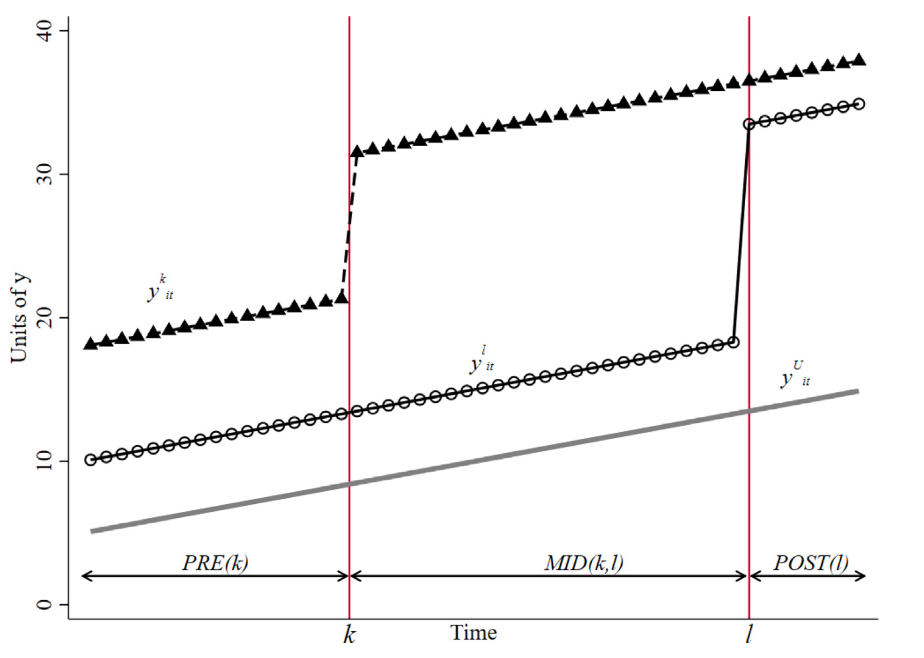
\includegraphics{goodman-baconDifferenceinDifferencesVariationTreatment2021_fig1.png}}
    \end{center}
    \medskip
    {\footnotesize Note: The figure plots outcomes in three timing groups: an untreated group, $U$; an early treatment group, $k$, which receives a binary treatment at $k = 34/100 T$; and a late treatment group, $l$, which receives the binary treatment at $l = 85/100 T$. The x-axis notes the three sub-periods: the pre-period for timing group $k$, $[1, k - 1]$, denoted by $PRE(k)$; the middle  period when timing group $k$ is treated and timing group $l$ is not, $[k, l - 1]$, denoted by $MID(k, l)$; and the post-period for timing group $l$, $[l, T]$, denoted by $POST(l)$. The treatment effect is $10$ in timing group $k$ and $15$ in timing group $l$.}
    \label{goodman-baconDifferenceinDifferencesVariationTreatment2021_fig1}
\end{figure}

By the Frisch-Waugh-Lovell theorem, $\wh{\b}^{DD}$ equals the univariate regression coefficient between $y_{it}$ and the treatment dummy with unit and time means removed:
\begin{equation}
    \label{3}
    \frac{\wh{C}\of{y_{it}, \wt{D}_{it}}}{\wh{V}^D} =\frac{\frac{1}{NT} \sum_i \sum_t y_{it} \wt{D}_{it}}{\frac{1}{NT} \sum_i \sum_t \wt{D}_{it}^2}.
\end{equation}
I denote grand means by $\ol{\ol{x}} = \frac{1}{NT} \sum_i \sum_t x_{it}$, and fixed-effects adjusted variables by $\wt{x}_{it} = \bp{x_{it} - \ol{x}_i} - \bp{\ol{x}_t - \ol{\ol{x}}}$.

One challenge in this setting has been to articulate how estimates of Equation \ref{2} compare the timing groups and times depicted in Figure \ref{goodman-baconDifferenceinDifferencesVariationTreatment2021_fig1}. We do, however, have clear intuition, for $2\times 2$ DD estimators in which one group's treatment status changes and another's does not. (These are just $2 \times 2$ DD estimators, so without additional assumptions discussed in Section 2 they cannot be interpreted as causal estimands.) In the three-group case we could form four such designs estimable by Equation (\ref{1}) on subsamples of timing groups and time periods. Figure \ref{goodman-baconDifferenceinDifferencesVariationTreatment2021_fig2} plots them. 

\begin{figure}[H]
    \noindent\caption{The four simple ($2 \times 2$) difference-in-differences estimates in the three group case.}
    \begin{center}
        \resizebox{1\textwidth}{!}{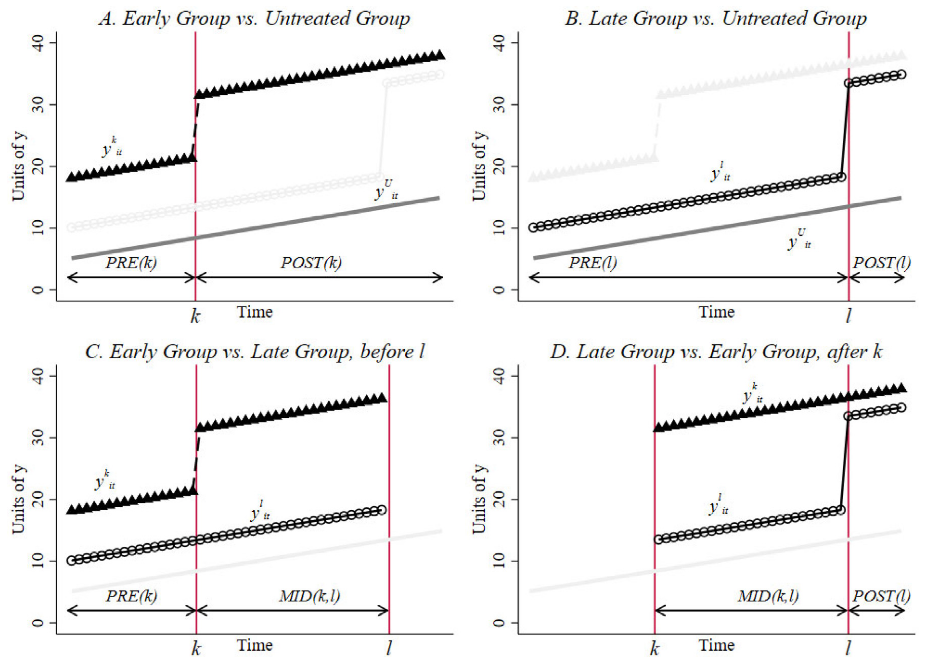
\includegraphics{goodman-baconDifferenceinDifferencesVariationTreatment2021_fig2.png}}
    \end{center}
    \medskip
    {\footnotesize Note: The figure plots outcomes for the subsamples that generate the four simple $2 \times 2$ difference-in-differences estimates in the three timing group case from Figure \ref{goodman-baconDifferenceinDifferencesVariationTreatment2021_fig1}. Each panel plots the data structure for one $2\times 2$ DD. }
    \label{goodman-baconDifferenceinDifferencesVariationTreatment2021_fig2}
\end{figure}

Panel A and B show that if we consider only one of the two treatment groups, the TWFE estimator reduces to the canonical case comparing a treated to an untreated group:
\begin{equation}
    \label{4}
    \wh{\beta}_{j U}^{2 \times 2} \equiv\left(\ol{y}_j^{{post }(i)}-\ol{y}_j^{{pre }(i)}\right)-\left(\ol{y}_U^{{post }(j)}-\ol{y}_U^{{pre }(j)}\right), \quad j=k, \ell .
\end{equation}
Note that I use $2 \times 2$ to refer to two time windows (here pre($j$) and post($j$)) instead of only two time periods. If instead there were no untreated units, the two way fixed effects estimator would be identified only by the differential treatment timing between groups $k$ and $\ell$. For this case, panels C and D plot two clear $2 \times 2$ DDs based on sub-periods when only one timing group's treatment status changes. Before $\ell$, the early units act as the treatment group because their treatment status changes, and later units act as controls during their pre-period. We compare outcomes between the window when treatment status varies, $mid(k, l)$, and timing group $k$'s pre-period, $pre(k)$: 
\begin{equation}
    \label{5}
    \wh{\b}_{k\ell}^{2\times 2, k} \equiv \bp{\ol{y}_{k}^{mid\of{k, \ell}} - \ol{y}_{k}^{pre\of{k}}} - \bp{\ol{y}_{\ell}^{mid\of{k, \ell}} - \ol{y}_{\ell}^{pre\of{k}}}.
\end{equation}
The opposite situation, shown in panel D, arises after $k$ when the later group changes treatment status but the early group does not. Later units act as the treatment group, early units act as controls, and we compare average outcomes between the periods $post\of{\ell}$ and $mid\of{k, \ell}$:
\begin{equation}
    \label{6}
    \wh{\b}_{k\ell}^{2\times 2, \ell} \equiv \bp{\ol{y}_{\ell}^{post\of{\ell}} - \ol{y}_{\ell}^{mid\of{k, \ell}}} - \bp{\ol{y}_{k}^{post\of{\ell}} - \ol{y}_{k}^{mid\of{k, \ell}}}.
\end{equation}
The already-treated units in timing group $k$ can serve as controls even though they are treated because treatment status does not change.

These simple DDs come from subsamples that relate to the full sample in two specific ways. First, each one uses a fraction of all $NT$ observations. The treated/untreated DDs in (\ref{4}) use two groups and all time periods, so their sample shares are $n_k + n_U$ and $n_{\ell} + n_U$. The treated/untreated DDs in (\ref{5}) and (\ref{6}) also use two groups but only some time periods, $\wh{\b}_{k\ell}^{2\times2, k}$ comes from timing group $\ell$'s pre-period so its share of all $NT$ observations is $\bp{n_k + n_{\ell}}\bp{1 - \ol{D}_\ell}$. $\wh{\b}_{k\ell}^{2\times2, \ell}$ comes from timing group $k$'s post-period so its share of all $NT$ observations is $\bp{n_k + n_\ell}\ol{D}_k$.

Second, each $2 \times 2$ DD is identified by how treatment varies in its subsample. The ``amount'' of identifying variation equals the variance of fixed-effects-adjusted $D_{it}$ from its subsample:
\begin{equation}
    \label{7}
    \wh{V}_{j U}^D \equiv n_{j U}\left(1-n_{j U}\right) \ol{D}_j\left(1-\ol{D}_j\right), \quad j=k, \ell
\end{equation}
\begin{equation}
    \label{8}
    \wh{V}_{k \ell}^{D, k} \equiv n_{k \ell}\left(1-n_{k \ell}\right) \frac{\ol{D}_k-\ol{D}_{\ell}}{1-\ol{D}_{\ell}} \frac{1-\ol{D}_k}{1-\ol{D}_{\ell}}
\end{equation}
\begin{equation}
    \label{9}
    \wh{V}_{k \ell}^{D, \ell} \equiv n_{k \ell}\left(1-n_{k \ell}\right) \frac{\ol{D}_{\ell}}{\ol{D}_k} \frac{\ol{D}_k-\ol{D}_{\ell}}{\ol{D}_k}
\end{equation}
where $n_{ab} = \frac{n_a}{n_a + n_b}$ is the relative size of timing groups in each pair. The first part of each pairwise variance measures how concentrated the timing groups is in the subsample. If $n_{jU}$ equals to zero or one, the variance goes to zero: there is either no treatment or no control group. The second part comes from \highlightP{when} the treatment occurs in each subsample. The $\ol{D}$ terms equal the variance of $D_{it}$ in each subsample's treatment group in its time window (thus the rescaling in \ref{8} and (\ref{9})). If $\ol{D}_j$ equals to zero or one the variance goes to zero: treatment does not vary over time.

\begin{theorem}[Difference-in-Differences Decomposition Theorem] \label{thm1}
    Assume that the data contain $k=1, \ldots, K$ timing groups of units ordered by the time when they receive a binary treatment, $k \in (1, T]$. There may be one timing group, $U$, that includes units that never receive treatment. The OLS estimate, $\wh{\b}^{DD}$, in a two-way fixed-effects regression (\ref{2}) is a weighted average of all possible two-by-two DD estimators.
    \begin{equation}
        \tag{10a} \label{10a}
        \hat{\beta}^{D D}=\sum_{k \neq U} s_{k U} \hat{\beta}_{k U}^{2 \times 2}+\sum_{k \neq U} \sum_{\ell>k}\left[s_{k \ell}^k \hat{\beta}_{k \ell}^{2 \times 2, k}+s_{k \ell}^{\ell} \hat{\beta}_{k \ell}^{2 x 2, \ell}\right] ,
    \end{equation}
    where the $2\times2$ DD estimators are:
    \begin{equation}
        \tag{10b} \label{10b}
        \wh{\beta}_{k U}^{2 \times 2} \equiv\left(\ol{y}_k^{{post}(k)}-\ol{y}_k^{{pre}(k)}\right)-\left(\ol{y}_U^{{post}(k)}-\ol{y}_U^{{pre}(k)}\right),
    \end{equation}
    \begin{equation}
        \tag{10c} \label{10c}
        \wh{\b}_{k\ell}^{2\times 2, k} \equiv \bp{\ol{y}_{k}^{mid\of{k, \ell}} - \ol{y}_{k}^{pre\of{k}}} - \bp{\ol{y}_{\ell}^{mid\of{k, \ell}} - \ol{y}_{\ell}^{pre\of{k}}},
    \end{equation}
    \begin{equation}
        \tag{10d} \label{10d}
        \wh{\b}_{k\ell}^{2\times 2, \ell} \equiv \bp{\ol{y}_{\ell}^{post\of{\ell}} - \ol{y}_{\ell}^{mid\of{k, \ell}}} - \bp{\ol{y}_{k}^{post\of{\ell}} - \ol{y}_{k}^{mid\of{k, \ell}}}.
    \end{equation}
    The weights are:
    \begin{equation}
        \tag{10e} \label{10e}
        s_{k U}=\frac{\left(n_k+n_U\right)^2 \overbrace{n_{k U}\left(1-n_{k U}\right) \ol{D}_k\left(1-\ol{D}_k\right)}^{\wh{v}_{k U}^D}}{\wh{V}^D}
    \end{equation}
    \begin{equation}
        \tag{10f} \label{10f}
        s_{k \ell}^k=\frac{\left(\left(n_k+n_{\ell}\right)\left(1-\ol{D}_{\ell}\right)\right)^2 \overbrace{n_{k \ell}\left(1-n_{k \ell}\right) \frac{\ol{D}_k-\ol{D}_{\ell}}{1-\ol{D}_{\ell}} \frac{1-\ol{D}_k}{1-\ol{D}_{\ell}}}^{\wh{V}_{k\ell}^{D, \ell}}}{\wh{V}_{k \ell}^D},
    \end{equation}
    \begin{equation}
        \tag{10g} \label{10g}
        s_{k \ell}^{\ell}=\frac{\left(\left(n_k+n_{\ell}\right) \ol{D}_k\right)^2 \overbrace{n_{k \ell}\left(1-n_{k \ell}\right) \frac{\ol{D}_{\ell}}{\ol{D}_k} \frac{\ol{D}_k-\ol{D}_{\ell}}{\ol{D}_k}}^{\wh{V}_{k\ell}^{D, \ell}}}{\wh{V}^D}.
    \end{equation}
    And 
    $$
    \sum_{k \neq U} s_{k U}+\sum_{k \neq U} \sum_{\ell>k}\left[s_{k \ell}^k+s_{k \ell}^{\ell}\right]=1 .
    $$
\end{theorem}

Theorem \ref{thm1} completely describes the sources of identifying variation in a TWFEDD estimator and their importance. With $K$ timing groups, one could form $K^2 - K$ ``timing-only'' estimates that either compare an earlier- to a later-treated timing group or a later- to earlier-treated timing group. With an untreated group, one could form $K$ $2\times2$ DDs that compare one timing group to the untreated group. Therefore, with $K$ timing groups and one untreated group, the DD estimator comes from $K^2$ distinct $2\times2$ DDs.

The weights on each $2\times2$ DD combine the absolute size of the subsample and the variance of the fixed-effects-adjusted treatment variable in the subsample. The first part is the size of the subsample squared. The second part of each weight is the subsample variance from Equations (\ref{7})-(\ref{9}), which comes from the relative size of the treatment and control groups and the timing of treatment. The variance is larger when the two timing groups are closer in size ($n_{kU} \approx 0.5$) and when treatment occurs closer to the middle of the time window.

\setcounter{equation}{10}

Theorem \ref{thm1} also shows how DD compares two treated groups. A two-group ``timing-only'' estimator is itself a weighted average of the $2\times2$ DDs plotted in panels C and D of Figure \ref{goodman-baconDifferenceinDifferencesVariationTreatment2021_fig2}:
\begin{equation}
    \label{11}
    \wh{\beta}_{k \ell}^{2 \times 2} \equiv \overbrace{\frac{\left(1-\ol{D}_{\ell}\right)^2 \wh{V}_{k \ell}^{D, k}}{\left(1-\ol{D}_{\ell}\right)^2 \wh{V}_{k \ell}^{D, k}+\ol{D}_k^2 \wh{V}_{k \ell}^{D, \ell}}}^{\mu_{k \ell}} \wh{\beta}_{k \ell}^{2 x 2, k}+\overbrace{\frac{\ol{D}_k^2 \wh{V}_{k \ell}^{D, \ell}}{\left(1-\ol{D}_{\ell}\right)^2 \wh{V}_{k \ell}^{D, k}+\ol{D}_k^2 \wh{V}_{k \ell}^{D, \ell}}}^{1-\mu_{k \ell}} \wh{\beta}_{k \ell}^{2 \times 2, \ell} .
\end{equation}
Both timing groups serve as controls for each other during periods when their treatment status does not change, and the weight assigned to the $2\times2$ terms comes from how large is their subsample and how large is their treatment variance. 

Theorem \ref{thm1} is not the only way to decompose the TWFEDD estimator. By grouping $2\times2$ terms according to the identifying variation (pre/post, treatment/control) that unites them, my ``group-level'' decomposition yields clear definitions for the weights and connects them to the features of the OLS estimation method.

The DD decomposition theorem is different from related results that decompose the TWFEDD estimand into a weighted average of treatment effect parameters with potentially negative weights. Theorem \ref{thm1} expresses the TWFEDD estimator as a weighted average of simpler estimators with strictly positive weights that sum to $1$. 

\section{Theory: What Parameter Does Dd Identify and Under What Assumptions}

Theorem \ref{thm1} relates the regression DD coefficient to sample averages, which makes it simple to analyze its statistical properties by writing $\wh{\b}^{DD}$ in terms of potential outcomes. Define $Y_{it}\of{k}$ as the outcome of unit $i$ in period $t$ when it is treated at $t_i = k$, and use $Y_{it}\of{t_i}$ to denote the treated potential outcomes under unit $i$'s actual treatment date. $Y_{it}\of{0}$ is the untreated potential outcome. If $t < t_i$ then $Y_{it}\of{t_i} = Y_{it}\of{0}$. The observed outcome is $y_{it} = D_{it} Y_{it}\of{t_i} + \bp{1-D_{it}}Y_{it}\of{0}$. Define the ATT for timing group $k$ at time $\tau \geq k$ (the ``group-time average treatment effect''):
$$
ATT_{k}\of{\tau} \equiv \E\bs{Y_{i\tau}\of{t_k^*} - Y_{i\tau}\of{0} \mid t_i = k}. 
$$
Because TWFEDD averages outcomes in pre- and post-treatment windows, I define the average $ATT_k\of{\tau}$ in a date range $W$ (with $T_W$ periods):
\begin{equation}
    \label{12}
    ATT_k\of{W} \equiv \frac{1}{T_W} \sum_{t \in W} \E\bs{Y_{it}\of{k} - Y_{it}\of{0} \mid t_i = k}.
\end{equation}
In practice, $W$ will represent post-treatment windows that appears in the $2\times2$ components. Finally, define the difference over time in average untreated potential outcomes as:
\begin{equation}
    \label{13}
    \D Y_k^0\of{W_1, W_0} \equiv \frac{1}{T_{W_1}} \sum_{t \in W_1} \E\left[Y_{i t}(0) \mid t_i=k\right]-\frac{1}{T_{W_0}} \sum_{t \in W_0} \E\left[Y_{i t}(0) \mid t_i=k\right].
\end{equation}
Applying this notation to the $2\times2$ DDs in Equations (\ref{4})-(\ref{6}), adding and subtracting average untreated outcomes for the treatment group yields the familiar results that (the probability limit of) each $2\times 2$ DD equals an ATT plus bias from differential trends:
\begin{equation}
    \tag{14a} \label{14a}
    \beta_{k U}^{2 \times 2}= {ATT}_k({post}(k))+\left[\Delta Y_k^0({post}(k), {pre}(k))-\Delta Y_U^0({post}(k), {pre}(k))\right]
\end{equation}
\begin{equation}
    \tag{14b} \label{14b}
    \beta_{k \ell, k}^{2 \times 2, k}= {ATT}_k({mid}(k, \ell))+\left[\Delta Y_k^0({mid}(k, \ell), {pre}(k))-\Delta Y_{\ell}^0({mid}(k, \ell), {pre}(k))\right]
\end{equation}
\begin{equation}
    \tag{14c} \label{14c}
    \begin{aligned}
        \beta_{k \ell}^{2 \times 2, \ell} = & {ATT}_{\ell}({post}(\ell))+\left[\Delta Y_{\ell}^0({post}(\ell), {mid}(k, \ell))-\Delta Y_k^0({post}(\ell), {mid}(k, \ell))\right] \\
        & - \left[{ATT}_k({post}(\ell))-{ATT}_k({mid}(k, \ell))\right]
    \end{aligned}
\end{equation}

\setcounter{equation}{14}

Note that the definition of common trends in (\ref{14a}) and (\ref{14b}) involves only untreated potential outcomes, but in (\ref{14c}) identification of $ATT_{\ell}\of{post\of{\ell}}$ additionally involves changes in average treatment effects in the already-treated control group. 

Substituting Equations (\ref{14a})-(\ref{14c}) into the DD decomposition theorem expresses the probability limit of the TWFEDD estimator (assuming that $T$ is fixed and $N$ grows) in terms of potential outcomes and separates the estimand from the identifying assumptions:
\begin{equation}
    \label{15}
    \plim_{\cvginf{N}} \wh{\b}^{DD} = \b^{DD} = VWATT + VWCT - \D ATT.
\end{equation}
The first term in (\ref{15}) is the interpretable causal parameter that TWFEDD can estimate, which I call the  ``\highlightB{variance-weighted average treatment effect on the treated (VWATT)}'':
\begin{equation}
    \label{15a} \tag{15a}
    V W A T T \equiv \sum_{k \neq U} \sigma_{k U} A T T_k({post}(k))+\sum_{k \neq U} \sum_{\ell>k}\left[\sigma_{k \ell}^k A T T_k({mid}(k, \ell))+\sigma_{k \ell}^{\ell} A T T_{\ell}({post}(\ell))\right].
\end{equation}
The $\sigma$ terms are probability limits of the weights in (\ref{10a}). $VWATT$ is a positively weighted average of ATTs for the treatment groups and post-periods across the $2\times2$ DDs that make up $\wh{\b}^{DD}$.

The second term, which I call the ``\highlightB{variance-weighted common trends (VWCT)}'' generalizes common trends to a setting with timing variation:
\begin{equation}
    \label{15b} \tag{15b}
    \begin{aligned}
        V W C T \equiv & \sum_{k \neq U} \sigma_{k U}\left[\Delta Y_k^0({post}(k), {pre}(k))-\Delta Y_U^0({post}(k), {pre}(k))\right] \\
        & +\sum_{k \neq U} \sum_{\ell>k}\left[\sigma_{k \ell}^k\left\{\Delta Y_k^0({mid}(k, \ell), {pre}(k))-\Delta Y_{\ell}^0({mid}(k, \ell), {pre}(k))\right\}\right. \\
        & \left.+\sigma_{k \ell}^{\ell}\left\{\Delta Y_{\ell}^0({post}(\ell), {mid}(k, \ell))-\Delta Y_k^0({post}(\ell), {mid}(k, \ell))\right\}\right].
    \end{aligned}
\end{equation}
Like $VWATT$, $VWCT$ is an average of the difference in counterfactual trends between pairs of timing groups and different time periods using the weights from the decomposition theorem. It captures the way that differential trends map to bias in (\ref{10a}). Note that one timing group's counterfactual trend affects many $2\times2$ DDs by different amounts and in different directions depending on whether it is the treatment or control group. While the mapping from trends to bias in a given $2\times2$ is clear, this result for a design with timing is new.

The last term in (\ref{15}) equals a weighted sum of the \highlightP{change} in treatment within each timing group's before and after a later treatment time:
\begin{equation}
    \label{15c} \tag{15c}
    \Delta A T T \equiv \sum_{k \neq U} \sum_{\ell>k} \sigma_{k \ell}^{\ell}\left[{ATT}_k({post}(\ell))-A T T_k({mid}(k, \ell))\right].
\end{equation}
Because the $2\times2$ estimators in Equation (\ref{14c}) already-treated groups as controls, they subtract average changes in their untreated outcomes and their treatment effects. $\D ATT$ equals zero if average treatment effect is constant, but when they are not, Equation (\ref{15c}) defines the resulting bias relative to $VWATT$ even when $VWCT=0$. $\D ATT$ is the source of the negative weights discussed in \citet{borusyakRevisitingEventStudyDesigns2024} and \citet{dechaisemartinTwoWayFixedEffects2020}. This does not mean that the research design is invalid. In this case, specifications such as an event-study, ``stacked DD'', or reweighting estimators may be more appropriate.

Units that are treated throughout the sample can only ever act as controls (in fact they enter into the decomposition theorem exactly like never-treated units), so if their treatment effects are chaning during the sample periods they will also contribute to $\D ATT$. The form of the weights suggests that changes in the treatment effects for always-treated units may dominate $\D ATT$. $2\times2$ DDs in which always-treated units are the control group use all time periods (as opposed to the smaller windows used in $\wh{\b}_{k\ell}^{\ell}$), so they get higher weight in (\ref{10a}). If their treatment effects are changing they can substantially bias TWFEDD away from VWATT. 

\subsection{Interpreting the TWFEDD Estimand}

When the treatment effect is a constant, $ATT_k\of{W} = ATT$, $\D ATT = 0$, and $VWATT = ATT$. The rest of this section assumes that $VWCT = 0$ and discuss how to intrepret $VWATT$ under different forms of treatment effect heterogeneity.

\subsubsection{Effects that vary across units but not over time}

If treatment effects are constant over time but vary across units, then $ATT_k\of{W} = ATT_k$ and we still have $\D ATT = 0$. In this case, DD identifies:
\begin{equation}
    \label{16}
    VWATT = \sum_{k \neq U} ATT_k \left[\overbrace{\sigma_{k U}+\sum_{j=1}^{k-1} \sigma_{j k}^k+\sum_{j=k+1}^K \sigma_{k j}^k}^{\equiv w_k^T}\right]
\end{equation}
$VWATT$ weights together the group-specific $ATT$s not by sample shares, but by a function of sample shares and treatment variance. The weights in (\ref{16}) are equal to the sum of the decomposition weights for all the terms in which timing group $k$ acts as the treatment group, defined as $w_{k^T}$.

In general, $w_k^T \neq n_k^*$, so $VWATT$ does not equal the sample $ATT$. Neither are the weights proportional to the share of time each unit spends under treatment, so $VWATT$ also does not equal the effect in the average treated period. The extent to which $VWATT$ differs from the ATT depends on the relationship between treatment effect heterogeneity and treatment timing in a given sample.

An easy way to gauge whether $VWATT$ differs from a sample-weighted $ATT$ is to scatter the weights from (\ref{16}), $w_k^T$, against each timing group's sample share among the treated, $\frac{n_k}{1-n_U}$. These two may be close if there is little variation in  treatment timing or if one timing group is very large. Conversely, weighting matters less if the $ATT_k$'s are similar, which one can evaluate by aggregating each timing group's $2\times2$ DD estimates from the decomposition theorem. Finally, one could directly compare TWFEDD to estimators that target a particular parameter of interest.

\subsubsection{Effects that vary over time but not across units}

Time-varying treatment effects shape Equation (\ref{15}) in two ways. First, they generate heterogeneity across the $2\times 2$ DDs that average over different post-treatment windows and up-weight short-run effects most likely to appear in the small windows between timing groups. These features typically make $VWATT$ different from the sample $ATT$. Second, time-varying effects bias estimates away from $VWATT$ because $\D ATT \neq 0$. 

To illstrate this point, Figure \ref{goodman-baconDifferenceinDifferencesVariationTreatment2021_fig3} plots a case where counterfactual outcomes are identical, but the treatment effect is a linear trend-break, $Y_{it}\of{k} = Y_{it}\of{0} + \phi \cdot \bp{t - t_i + 1}$. $\wh{\b}_{k\ell}^{2\times2, k}$ uses timing group $\ell$ as a control group during its pre-period and identifies the $ATT$ during the middle window in which treatment status varies: 
$$
ATT\of{mid\of{k, \ell}} = \phi \cdot \frac{\ell - k + 1}{2}.
$$
$\wh{\b}_{d\ell}^{2\times2, \ell}$, however, is biased for $ATT\of{post\of{\ell}}$ because the control group ($k$) experiences a trend in outcomes due to it growing treatment effect:
\begin{equation}
    \label{17}
    \wh{\beta}_{k \ell}^{2 \times 2, \ell}=\overbrace{{A T T_{\ell}({post}(\ell))}}^{\phi \frac{T-\ell+1}{2}}-\overbrace{\phi \frac{T-k+1}{2}}^{\Delta A T T /\left(1-\mu_{k \ell}\right)}=\phi \cdot \frac{k-\ell}{2} \leq 0 .
\end{equation}
This bias feed though ot $\beta_{k\ell}^{2\times2}$ to the relative weight on the $2\times 2$ terms:
\begin{equation}
    \label{18}
    \wh{\beta}_{k \ell}^{2 x 2}=\phi \frac{\left[\left(\sigma_{k \ell}^k-\sigma_{k \ell}^{\ell}\right)(\ell-k)+1\right]}{2} .
\end{equation}

The entire two-group timing estimate can be wrong signed if there is sufficiently more weights on $\wh{\beta}_{k \ell}^{2 \times 2, \ell}$ than $\wh{\beta}_{k \ell}^{2 \times 2, k}$. Summarizing time-varying effects using Regression (\ref{2}) yields estimates that are too small or even wrong-signed,  and should not be used to judge the meaning or plausibility of effect sizes.


\begin{figure}[H]
    \noindent\caption{Difference-in-Differences estimates with variation in timing are biased when treatment effects vary over time.}
    \begin{center}
        \resizebox{0.7\textwidth}{!}{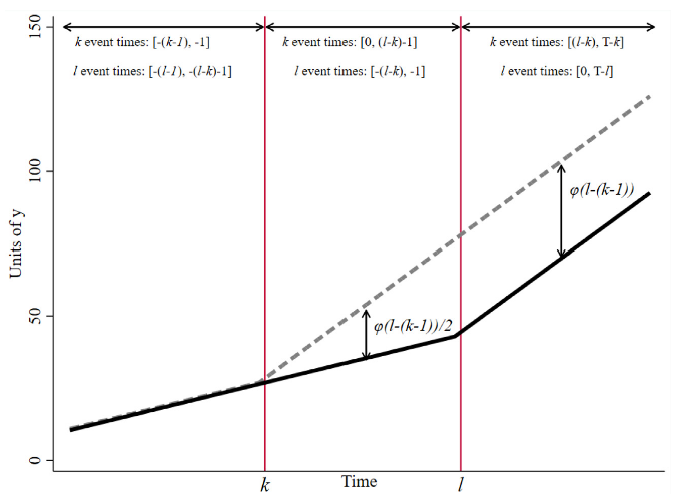
\includegraphics{goodman-baconDifferenceinDifferencesVariationTreatment2021_fig3.png}}
    \end{center}
    \medskip
    {\footnotesize Note: The figure plots a stylized example of a timing-only DD set up with a treatment effect that is a trend-break rather than a level shift. The trend-break effect equals $\phi \cdot \bp{t-t_i + 1}$. The top of the figure notes which event-times lie in the $pre\of{k}, mid\of{k, \ell}$, and $post\of{\ell}$ periods for each unit. The figure also notes the average difference between timing groups in each of these periods. In the $mid\of{k,\ell}$ period, outcomes differ by $\frac{\phi}{2} \bp{\ell - k + 1}$ on average. In the $post\of{\ell}$ period, however, outcomes had already been growing in the early group for $\ell - k$ periods, and so they differ by $\phi \bp{\ell - k + 1}$ on average. The $2\times2$ DD that compares the later-treated group to the earlier-treated group is biased and, in the linear trend-break case, weakly negative despite a positive and growing treatment effect.}
    \label{goodman-baconDifferenceinDifferencesVariationTreatment2021_fig3}
\end{figure}

Note that this bias is specific to a single-coefficient specification. More flexible event-study specifications may not suffer from this problem. 

\subsection{What Is the Identifying Assumption for $VWATT$?}

The preceding analysis maintained the assumption of \highlightP{equal} counterfactual trends across timing groups, but (\ref{15}) shows that when $\D ATT = 0$ identification of $VWATT$ only requires $VWCT = 0$. Assuming linear average untreated potential outcome trends 
$$
\ol{Y}_{kt}\of{0} - \ol{Y}_{k, t-1}\of{0} = \D Y_k^0
$$
for all $t$, leads to a convenient and intuitive approximation to $VWCT$ as an average of each timing group's average trend in $Y\of{0}$ weighted by the difference between its weight as a treatment group $w_k^T$ from Equation (\ref{16}) and a similar term measuring its weight as a control group:
\begin{equation}
    \label{19}
    \begin{aligned}
    V W C T & \approx \sum_{k \neq U} \Delta Y_k^0\left[\left(\sigma_{k U}+\sum_{j=1}^{k-1} \sigma_{j k}^k+\sum_{j=k+1}^K \sigma_{k j}^k\right)-\left(\sum_{j=1}^{k-1} \sigma_{j k}^j+\sum_{j=k+1}^K \sigma_{k j}^j\right)\right]-\Delta Y_U^0 \sum_{k \neq U} \sigma_{k U} \\
    & =\sum_k \Delta Y_k^0\left[w_k^T-w_k^C\right]
    \end{aligned}
\end{equation}

Equation (\ref{19}) generalizes the definition of common trends to the timing case and shows how a given timing group's counterfactual trend biases the overall estimate. To illustrate, assume there is a positive differential trend in timing group $k$ only: $\D Y_k^0 > 0$. This will bias $\wh{\b}_{kU}^{2\times2}$ by $\D Y_k^0$ which gets a weight of $\s_{kU}$ in the full estimation. In $2\times2$ DDs based on timing, however, biases offset each other. Take the comparisons to timing group $1$, for example. When timing group $k$ is the  treatment group in $\wh{\b}_{1k}^{2\times2, k}$, the bias equals $\D Y_k^0$ and is weighted by $\s_{1k}^{k}$. When timing group $k$ is the control group in $\wh{\b}_{1k}^{2\times2, 1}$,  the bias equals $-\D Y_k^0$ and is weighted by $\s_{1k}^{1}$. On net the bias in $\wh{\b}_{1k}^{2\times2}$ is ambiguous: $\D Y_k^0 \bp{\s_{1k}^{k} - \s_{1k}^{1}}$.

Similar expressions hold for the comparison of timing group $k$ to every other group, and the total weight on each timing group's counterfactual trend equals the difference between the total weight it gets when it acts as a treatment group, $w_{k}^{T}$ from Equation (\ref{16}), minus the total weight it gets when it acts as a control group, $w_{k}^{C}$. This difference is a new result that maps (linear) differential trends to bias.

Figure \ref{goodman-baconDifferenceinDifferencesVariationTreatment2021_fig4} plots $w_{k}^{T} - w_{k}^{C}$ as a function of $\ol{D}$ assuming equal group sizes. Units treated in the middle of the panel have high treatment variance and get a lot of weight when they act as the treatment group, while units treated toward the ends of the panel get relatively more weight when they act as controls. As $k$ approaches $1$ or $T$, $w_{k}^{T} - w_{k}^{C}$ becomes negative which means that some timing groups effectively act as controls. This defines ``the'' control group in timing-only designs: all timing groups are controls in some terms, but the earliest and/or latest units necessarily get more weight as controls than treatments.

\begin{figure}[H]
    \noindent\caption{Weighted common trends: The treatment/control weights as a function of the share of time spent under treatment.}
    \begin{center}
        \resizebox{0.7\textwidth}{!}{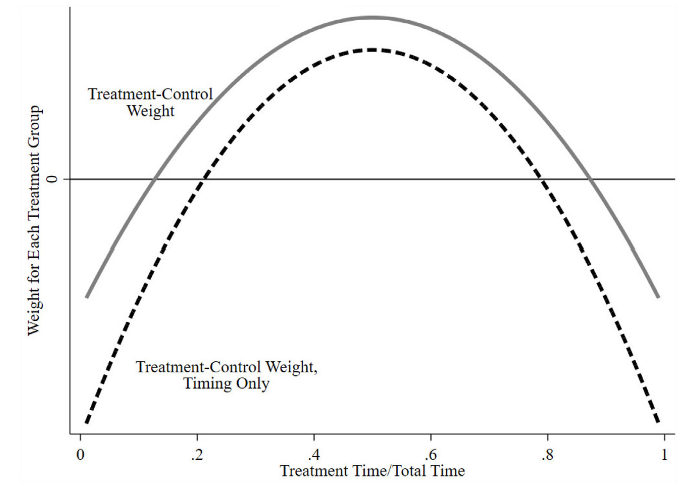
\includegraphics{goodman-baconDifferenceinDifferencesVariationTreatment2021_fig4.png}}
    \end{center}
    \medskip
    {\footnotesize Note: The figure plots the weights that determine each timing group's importance in the weighted common trends expression in Equation (\ref{19}).}
    \label{goodman-baconDifferenceinDifferencesVariationTreatment2021_fig4}
\end{figure}

\bibliography{\CiteReference}

\end{document}
